\begin{center}
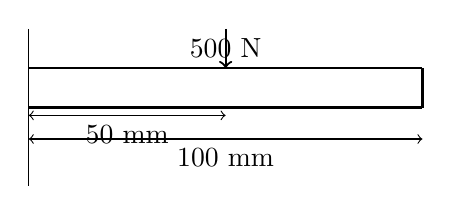
\begin{tikzpicture}
    % Draw the beam
    \draw[thick] (0,0.5) -- (5,0.5);
     \draw[thick] (0,0) -- (5,0);
     \draw[thick] (5,0) -- (5,0.5);
    \draw (0,1) -- (0,-1); % Fixed support
    


    % Draw the point load
    \draw[thick, ->] (2.5,1) -- (2.5,0.5) node[right,above] {$500$ N}; % Load arrow and label
    
    % Labels for dimensions
    \draw[<->] (0,-0.4) -- (5,-0.4) node[midway, below] {$100$ mm}; % Beam length label
    \draw[<->] (0,-0.1) -- (2.5,-0.1) node[midway, below] {$50$ mm}; % Beam length label
\end{tikzpicture}
\end{center}
